\begin{comment}
    \begin{itemize}
        \item Application of regression analysis? (why?)
        \item introduction of regression model
        \item description of model fitting?  (mcmc description, time?)
        \item results (emergent clusters?)
    \end{itemize}
\end{comment}

Let $i$ iterate over observations, $s$ iterate over sites (locations), and $\ell$ iterate over 
    dimensions of $\bm{\theta}$
\begin{equation}
    \begin{aligned}
        \bm{y}_i &\sim \mathcal{PG}(\bm{y}\mid f(\bm{x}_i^T\bm{\theta}_i + \bm{\varepsilon}), \bm{1})\\
        \theta_i &\sim G\\
        G &\sim \mathcal{PY}(G\mid\eta, d, G_0)
    \end{aligned}
    ~\hspace{2cm}
    \begin{aligned}
        G_0 &= \mathcal{N}(\bm{\theta} \mid \mu, \Sigma)\\
        \varepsilon_{\ell} &\sim \mathcal{N}(\varepsilon \mid 0, \sigma_{\epsilon})\\
        \mu,\Sigma &\sim \mathcal{NIW}(\mu,\Sigma\mid \bm{0}, \kappa, \nu, \psi)
    \end{aligned}
\end{equation}

\begin{figure}[ht]
    \centering
    \caption{Posterior predictive distribution under a \emph{fully specified} model, colored 
        by cluster.  Left is the regressors, $\bm{X}$.  Center is after linear transformation, 
        projected onto unit simplex, $T_{1}(\bm{X}\bm{\theta})$.  Right is posterior predictive 
        distribution, $T_1(\bm{X}\bm{\theta}^*).$\label{fig:simreg}}
    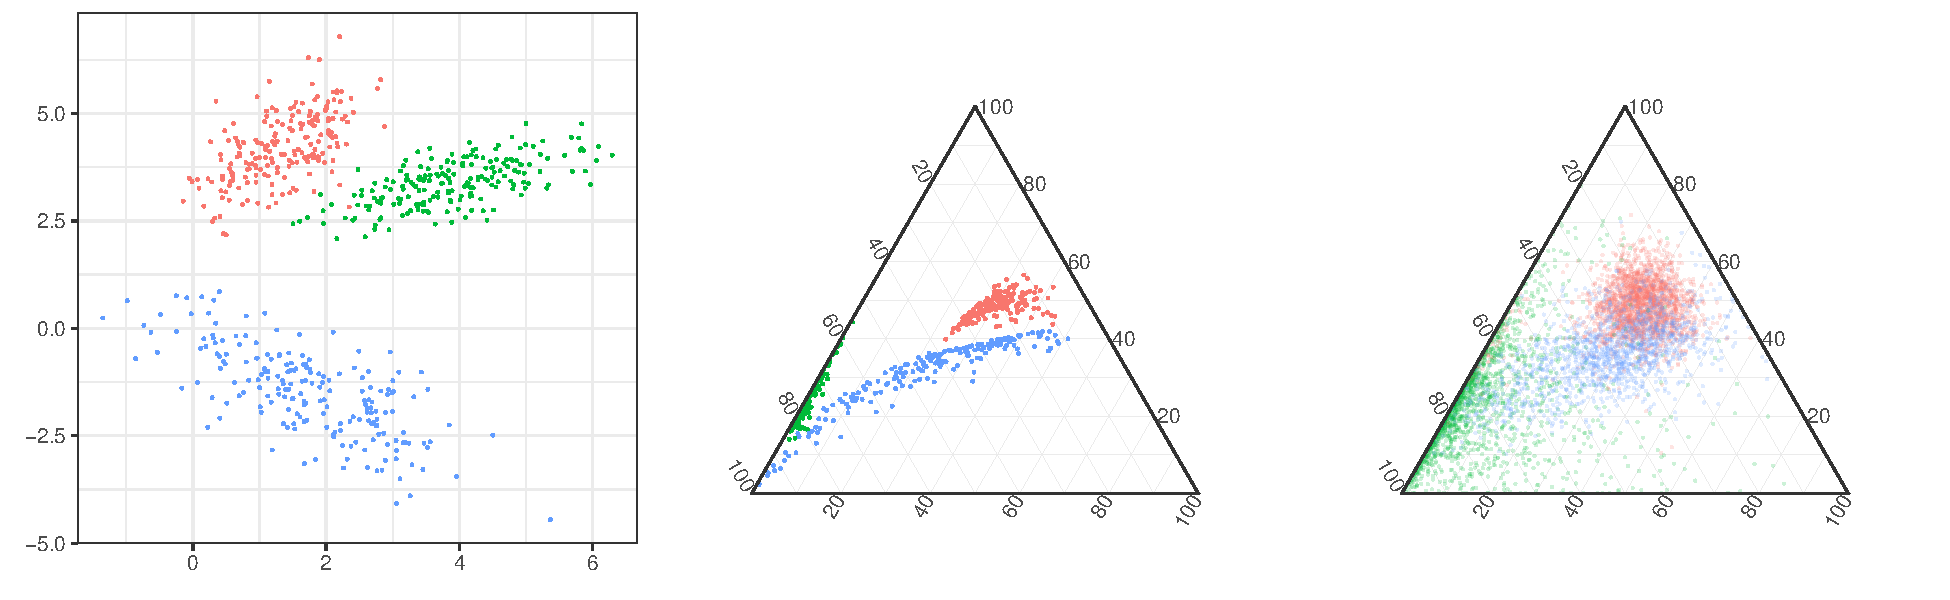
\includegraphics[width = \textwidth]{plots/simulated_reg}
\end{figure}

The term $\bm{x}_i$ is overloaded.  For $\bm{y}_{is}$ ($i$th observation, $s$th location), 
    $\bm{x}_{is}$ (covariates associated with observation $i$ at location $s$) include 
    $\bm{x}_{i,\text{obs}}$, the parameters under which the $i$th storm 
    was modelled; $\bm{x}_{s,\text{loc}}$, information pertaining to the $s$th location, such
    as latitude and longitude; and $\bm{x}_{is,\text{int}}$, any interaction thereof.  Currently
    this consists of a single term, the linear interaction between latitude of storm eye at landfall, 
    and latitude of location.